\documentclass{scrartcl}
%common packages
\usepackage{hyperref}
\usepackage{amsmath}
\usepackage{amsfonts}
\usepackage{amssymb}
\usepackage{amsthm}
\usepackage{caption}
\usepackage{algorithm}
\usepackage[noend]{algorithmic}
\usepackage{natbib}
\usepackage{graphicx}

%some common comman definitions
\newcommand{\R}{\mathbb{R}}
\newcommand{\N}{\mathbb{N}}
\newcommand{\expected}{\mathbb{E}}
\newcommand{\bigO}{\mathcal{O}}
\newcommand{\smallo}{\textit{\textbf{o}}}

\title{Efficient First Order Inductive Learner\\ on Spark}
\subtitle{Lab Report: Distributed Big Data Analytics, 2017}
\date{}

\author{Georgiy Shurkhovetskyy, Eskender Haziiev}

\begin{document}

\maketitle

\begin{abstract}
The presented report deals with realization of First Order Inductive Learner.
The  work is based on the approach by J.R. Quinlan and is developed using Spark  framework.
A prediction rule in a form of a set of Horn clauses for a target relation that consistent
 with given positive examples and not cover any given negative examples is displayed result. Each example is given as positive or negative tuple.
As input data the application receives an information about the name and a set of positive and negative tuples of target predicate,  a list of  names and sets of positive tuples of predicates that can appear in a right-hand side of the rule. Three successful experiments were carried out.
\end{abstract}

\section{Problem definition}

\subsection{Introduction}

Learning theory considers any object as fixed collection of attributes   and there is solved a problem on belonging of this object to one of a bounded number of mutually exclusive classes.
Using inductive approach the above problem is clarified as follows. Suppose we have an information on belonging some training set of objects having the similar structure to one of two mutually exclusive classes. It is necessary to find a rule for predicting the class of an unseen object having the similar structure of a set of the attributes. Note that a set of object attributes does not have to coincide with the complete set of attributes and can only be subset of the last one.

Several methods are used to solve such problem. One of them (so-called a divide-and-conquer method) is based on a construction of a decision tree (DT) from a given training set, then if-then rules are extracted from  DT. An algorithm consists of two operations: a selection of a test based on one attribute and a separation of the training set into subsets  corresponding to one of the mutually exclusive results of this test. Then these operations are repeated to obtained subsets. The process is ended when all examples from each obtained subsets are belonged to a single class (i.e. labeled as a leaf). However, the construction of a compact DT strongly depends on the successful choice of the test, the algorithm is greedy and takes a lot of time \citep{Quinlan1990}.

To get rules from a training set an inductive method (so-called a covering method, AQ family) directly uses the concept of separate and conquers. This approach includes: a finding of a conjunction of conditions that is satisfied by some objects in the target class, but no objects from another class (in fact, this is a test); appending of obtained conjunction in disjunctive logical expression and remove all objects that satisfy it. The procedure repeats if there are still remaining objects of the target class. The \textrm{"}bottleneck\textrm{"} of this approach is based on its dependence on specific training examples \citep{Quinlan1990}.

Using concrete example (see network at Figure 1) \citet{Quinlan1990}  showed the principal weakness of described above methods and suggested  new inductive approach realized in FOIL (First Order Inductive Learner).
FOIL  is a system which learns function-free Horn clause definitions from data expressed as relations in terms of itself and other relations. \citet{Quinlan1990} presented the results on six problems addressed by other learning systems, see more in \citep{Quinlan1993, Quinlan1995}.
\begin{figure}[h!] \centering
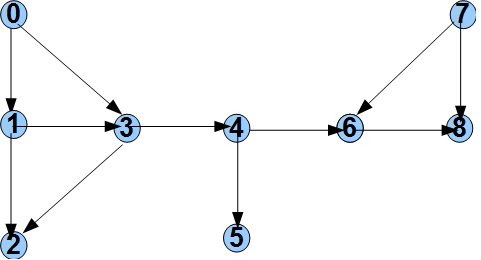
\includegraphics[bb =0 0 481 260,scale =0.3]{foil1.png}
\caption{Illustrated example by \citet{Quinlan1990}.}
\end{figure}
Noted that \citet{Muggleton1994} pointed out that FOIL system \textrm{"}relates to the greedy TDIDT-algorithms and the AQ family of algorithms...was the first widely known demonstration that the first order learning ... works efficiently on a broad range of problems involving large and noisy datasets\textrm{"}.

Our report deals with the following problem: \emph{using Spark framework to realize FOIL
which finds a learning rule in form of
 a set of Horn clauses for the target relation that consistent
 with given positive examples and not cover any given negative examples.}

It should be noted that \emph{the desired application is of interest for a Big Data problem} for the following reasons.  The Big Data problems usually handles large amounts of input data in the learning process. The effectiveness of the process is directly related to the representation of the training data and a result. The FOIL as inductive approach allows to derive from a given training data a learning rule in the analytical form, namely as  Horn clauses. A brief analytical form of the obtained learning rule allows us  to  obtain a prediction on a belonging to one or another mutually exclusive class for any unseen object quickly enough.


\subsection{Learning Logical Definitions from Relations:
concepts  and algorithm}

Based on \citep{Quinlan1990, Quinlan1993} we will outline the basic concepts and the main ideas of learning logical definitions from relations.

Most often an object may belong to one of two classes
or we have to predict whether an object belongs to some class.
To predict the learning rules represented by Horn clauses can be used.
So we discuss a subject of present report  namely for this case.
%% This  assumption does not restrict the generality and  it is made for the sake of simplicity of exposition.

FOIL input usually consists of information on several relations. One of them is target relation and its Horn clauses representation is to be founded.

Preliminarily let us give some basic definitions.

\textbf{Definition 1}.
A literal $L$ may be unnegated predicate $P$ or negated predicate $\neg{P}$.

\textbf{Definition 2}.
A claus body is a conjunction of literals.

\textbf{Definition 3}.
A clause head is predicate.

\textbf{Definition 4}.
A Horn clause consists of a clause head and a clause body in a form
\begin{equation}\label{eq0}
P\leftarrow L_1,L_2,..., L_n\quad,
\end{equation}
where each $L_i$, $i=1,2,\ldots, n$, is literal.

\textbf{Definition 5}.
A learning rule for predicate $P$ is
 a collection of Horn clauses each with head $P$.

Note that Definition 1 and Definition 4 are important
for recursive definition of predicate
 (it is seen when in \eqref{eq0}  we use $P$ in clause body instead some $L_i$).

The predicates can be defined \emph{extensionally} as a list of tuples
for which the predicate is true, or \emph{intensionally} as a set of Horn clauses (using them we can compute whether the predicate is true).


\textbf{Definition 6}.
$k$-tuple is a finite sequence of $k$ constants,
denoted by $<a_1, a_2, \ldots, a_k>$.

Below we also will use a short term $tuple$ instead a term $k-tuple$.

\textbf{Definition 7}.
A tuple satisfies a rule if it satisfies one of the Horn clauses
of this rule.

For every relation a set of the tuples  which
 belong to this relation (denoted by $\oplus$) is given.
  So such set is given for target relation too.

For example represented at Figure 1 the relation $linked-to(X,Y)$
may be given:
\begin{multline}\label{eq1}
linked-to (X,Y) =
\oplus\{<0,1>, <0,3>, <1,2>, <3,2>, <3,4>,\\ <4,5>, <4,6>, <6,8>, <7,6>, <7,8>\}.
\end{multline}
Each tuple $<X,Y>$ in \eqref{eq1} means that node $X$ directly
linked (connected)
to node $Y$.

For a target relation a set of $\oplus$ tuples is also given.
A set of the tuples not belonging (denoted by $\ominus$) to the target relation
 may be given.
The statement is introduced: if some tuple is
not included in set $\oplus$ tuples
 then it is $\ominus$ tuple.

Let a target relation be $can-reach(X,Y)$
which means that exists or not exists a path from node $X$ to node $Y$. Then we have for
above example:
\begin{multline}\label{eq3}
can-reach(X,Y)=\ominus\{<0,0>, <0,7>,  \\
<1,0>,<1,1>,<1,3>, <1,4>,<1,5>,<1,6>,<1,7>,<1,8>,<2,0>,\\
 <2,1 >, <2,2 >, <2,3 >, <2,4 >, <2,5 >, <2,6 >, <2,7 >, <2,8 >,< 3,0>, \\
 <3,1 >, <3,3 >, <3,7 >,  < 4,0>, <4,1 >, <4,2 >, <4,3 >, <4,4 >, <4,7 >, \\
  <5,0>, <5,1 >, <5,2 >, <5,3 >, <5,4 >, <5,5 >, <5,6 >, <5,7 >, <5,8 >,\\
  <6,0>, <6,1 >, <6,2 >, <6,3 >, <6,4 >, <6,5 >, <6,6 >, <6,7 >,< 7,0>,\\
   <7,1 >, <7,2 >, <7,3 >, <7,4 >, <7,5 >,  <7,7 >,<8,0>,<8,1 >,<8,2 >, \\
    <8,3 >, <8,4 >, <8,5 >, <8,6 >, <8,7 >, <8,8 >,\}.
\end{multline}
\begin{multline}\label{eq2}
can-reach(X,Y)=\oplus\{<0,1>, <0,2>, <0,3>, <0,4>,<0,5>, <0,6>, \\
\qquad\quad\qquad\qquad<0,8>,<1,2>,<3,2>, <3,4>,<3,5>, <3,6>, <3,8>,\\
<4,5>, <4,6>,<4,8>,<6,8>, <7,6>, <7,8>\}.
\end{multline}




\textbf{\emph{The problem definition:}} To find a learning rule
as a set of Horn clauses  for a target relation
 that consistent with all given $\oplus$ tuples and not cover any given $\ominus$ tuples.


\section{Approach}

In this project we follow the algorithm FOIL described above and presented in Table 1.
It is not intended to apply any parallelization of the process. For implementation the Spark framework and Scala programming language should be used. It is intended to use training data based on \citep{Horvath2016} and \citep{Quinlan1990}.

\citet{Pazzani1992} formulated two designs of the FOIL algorithm,
one of them is presented below in Table 1.

\begin{tabular}{c}

\end{tabular}

Table 1. FOIL Design II (by \citet{Pazzani1992}).

\begin{tabular}{|l|l|} %% viravnivanie: r po pravomu krau   c po centru
  \hline
  % after \\: \hline or \cline{col1-col2} \cline{col3-col4} ...
  1 & Let Pred be the predicate to be learned  \\
  \hline
  2 & Let Pos be the positive examples  \\
  \hline
  3 & Until Pos is empty do:  \\
  \hline
  4 &   \qquad Let Neg be the negative examples \\
  \hline
  5 &   \qquad Set Body to empty \\
  \hline
  6 &   \qquad Let Old be those variables used in Pred \\
  \hline
  7 &   \qquad CallLearnClauseBody \\
  \hline
  8 &   \qquad Add Pred $\leftarrow$ Body to the rule \\
  \hline
  9 &   \qquad Remove from Pos all examples that satisfy the Body \\
  \hline
    7a & Procedure CallLearnClauseBody  \\
  \hline
  7b & \qquad Until Neg is empty do:  \\
  \hline
  7c & \qquad\qquad For each predicate-name P  \\
  \hline
  7d & \qquad\qquad For each variabilization L of P  \\
  \hline
  7e & \qquad\qquad Compute information gain of L and its negation \\
  \hline
  7f & \qquad\qquad Select literal L with most information gain \\
  \hline
  7g & \qquad\qquad Conjoin L to Body  \\
  \hline
  7h & \qquad\qquad Add any new variables to Old  \\
  \hline
  7i & \qquad\qquad Let Pos be all extensions of Pos that are satisfied by the literal \\
  \hline
  7j & \qquad\qquad Let Neg be all extensions of Neg that are satisfied by the literal  \\
  \hline

 \end{tabular}

\vspace{6pt}

FOIL has two levels of a processing: an \emph{outermost level} and a \emph{inner level}.

\emph{At the outermost level} FOIL starts with a training set containing
all $\oplus$ and $\ominus$ tuples,
 constructs a function-free Horn clause which consistent with some $\oplus$ tuples,
removed the covered $\oplus$ tuples from the training set
and continues with the search for next clause.
This operation is ended when the set of $\oplus$ tuples becomes empty.

\emph{At the inner level} FOIL constructs current Horn clause in form \eqref{eq0}.
The current clause is expands by adding new literals to the body.
In general inner loop starts with assignment current training set $T_1$
to training set and  initialization $i = 1$;
then while $T_i$ contains $\ominus$ tuples a new literal $L_i$ is found
and is added to the body of current clause,
new current training set $T_{i+1}$ is generated based only on
 tuples from $T_i$ which are satisfied to literal $L_i$,
 variable $i$ is incremented and inner loop is repeated.
 The inner loop is ended when set of $\ominus$ tuples in $T_i$ becomes empty.


The operations 7c--7f in
 CallLearnClauseBody
select one of the possible literals.
The having greatest positive gain literal is added to a current clause body.
At each $i$-nd iteration of the inner loop the literal $L_{i}$
 is looking for one of the possible literals:
 \begin{equation}\label{eq4}
gain (L_{i})=n_i^{\oplus\oplus} \cdot (I(T_i)-I(T_{i+1})),\quad
I(T_i)=-\log_2 (n_i^\oplus/(n_i^\oplus+n_i^\ominus)),
\end{equation}
where $n_i^\oplus$ --- a number of $\oplus$ tuples in $T_i$,
$n_i^\ominus$ --- a number of $\ominus$ tuples in $T_i$,
$n_i^{\oplus\oplus}$ --- a number of the $\oplus$ tuples in $T_i$
 which  are represented by one or more tuples in $T_{i+1}$.

The construction of new training set is also nontrivial, see 7h-7j.
New training set consists of
 the $\oplus$ and $\ominus$ tuples which may have a larger length
if a new variable was appeared in the clause body.
The following operations are realized: for each tuple $t$ in $T_i$ and for each binding $b$ of any new variables
introduced by the literal $L_i$ do:
if the tuple $<t,b>$ satisfies $L_i$
then add $<t,b>$ to $T_{i+1}$
with the same label ($\oplus$ or $\ominus$) as $t$.



\section{Implementation}

For the implementation of described above algorithm Scala programming language and Spark framework were used.
The predicates were generated as follows: $predicate(tuples)$, where $predicate$ is predicate name, $tuples$ is a list of the tuples for this predicate. The background knowledge is a list of $predicate(tuples)$ characterizing positive examples of predicates which can appear as literals on the right-hand side of the Horn clause.

To generate a learning rule  we use the basic methods of our own class $KnowledgeBase$:

1. $load$ which  loads data from input stream and store the sets of positive examples and negative examples of target predicate,  background knowledge $\mathcal{B}$, as $DataSource$ objects within class fields (in fact $load$ enters a training data);

2. $foil$  runs FOIL algorithm which uses the sets of positive examples and negative examples and background knowledge and obtains the  rules.

Describing the work of the method $foil$ it should be noted that the sequence of operations is performed:

2.1. $generateCandidates$  generates list of $candidates$  with all possible combinations of variables from background knowledge predicates;

2.2. for each $PositiveExample$ until  $PositiveExamples\neq \emptyset$ a set $NegativeExamples$ is taken;

    2.2.1. for each $NegativeExample$ until $NegativeExamples\neq \emptyset$  every candidate from $candidates$ is taken;

    2.2.2. $findMaximalClause$ finds \textrm{"}maximal\textrm{"}  Horn clause, i.e. finds a predicate having maximal weighted gain calculated by formula \eqref{eq4};

    2.2.3. a clause body is updated by concatenation of the predicate having maximal weighted gain.

2.3. the generated rule is displayed.

Now consider method $findMaximalClause$  having as Input $targetPredicate$ (i.e. left-hand side of the rule), $bodyPredicates$ (i.e. already generated right-hand side of the rule), the sets $PositiveExamples$ and $NegativeExamples$. As mentioned above this method has as Output a predicate having maximal weighted gain calculated by \eqref{eq4}. $findMaximalClause$ executes the call $foilAlgorithm$; and returns set of the tuples covered by the rule and weighted gain, obtained from $n^+$, $n^-$ and $n^{++}$.

The method $foilAlgorithm$ is designed for check tuples in FOIL algorithm. As Input it has $targetTuples$ to be checked, $targetPredicate$ in left-hand side of the rule, $bodyPredicates$ already generated right-hand side of the rule. As Output $foilAlgorithm$  obtains Scala tuple containing calculated $n^+$, $n^-$ and $n^{++}$, and the set of the tuples covered by the rule.

\subsection {Parallelization }

In FOIL algorithm number of predicates and number of possible variable combinations happen to be the drivers of complexity of the entire approach to learn the rules. This makes precisely the step which succeed generation of candidates to be the perfect candidates for parallelization. After we have built our pool of candidates, we resort to distributive capabilities of Spark to achieve parallelization.

In particular, in method $foil$ we convert $candidates$ into a Spark-ready data object - Resilient Distributed Dataset (RDD). At this point it contains list of predicates available. We define $flatMap$ operation on our existing RDD. It applies specified function of every element of given RDD and returns a new one. In this particular case we expand all the variable candidates for a predicate so that later one we could easily calculate gain for every combination.

Next step involves evaluation every candidate defined by predicate and variable combination. We define another $map$-based transformation with a function which calculates gain for every element in the RDD. $Map$ transformation is different from $flatMap$ in that it does not return an array, but only a single unit. This fits our needs perfectly at this point since we have already expanded the candidates' list and are only interested in 1:1 mapping of candidate to its gain.

Final step is reduction which ultimately triggers the transformations specified previously ($flatMap$ and $map$). Function based on which it executes is associative and binary - it takes two arguments and returns one. In our case it is implemented in comparator-like fashion as we are interested in being left with just one record in a resulting RDD - the one which holds configuration with the highest gain. Function $getMaxGain$ does exactly that by first retrieving gain value from the tuples and then comparing it to gain of opponent unit.

After having executed $reduce$ action operator we are free to extract the calculated values and suggest the rules.

\section{Evaluations}

The efficiency of our application is estimated by three indicators. The first and second ones are connected with the evaluation of the correctness of the obtained result, i.e. whether the obtained rile is consistent with the given training data. Here we analyzed a proportion of positive examples and a proportion of negative examples that are covered by the obtained rule (in percentage terms). It is obvious that these indicators satisfy metrics properties and the application can be evaluated as  \textrm{"}efficient\textrm{"} if it has a high first rate and a low second one.
The third indicator characterizes the speed of data processing. Here we analyzed a running time of program (in seconds). The application can be evaluated as  \textrm{"}efficient\textrm{"} if it has a low running time.

Three experiments were running in Spark framework and the learning rules in form \eqref{eq0} were obtained.
In the first experiment we used training data from \citep{Horvath2016}. The target relation is 2-ary predicate $daughter(X_1,X_2)$;  2-ary predicate $parent(X_1,X_2)$ and 1-ary predicate $female(X)$ can be used in learned clause body. The predicates names are replaced by initial letters $d$, $p$ and $f$ correspondingly.  The training data is following:
\begin{multline}\label{eq13a}
\!\!\!\!\mathcal{B}= \{p(tom, bill), p(tom, emily), p(ann, tom), p(ann, mary),
f(emily), f(mary), f(ann)\},\\
PositiveExamples= \{d(emily, tom), d(mary, ann) \},\\
NegativeExamples= \{ d(emily, ann), d(tom, ann)\}.
\end{multline}
The method $generateCandidates$ uses the literal candidates:
\begin{multline}\label{eq13b}
candidates=\{
p(X_2, X_1), p(X_1, X_2), p(X_1, Y_1), p(Y_1, X_1), p(X_2, Y_1), p(Y_1, X_2),\\ p(X_1, X_1), p(X_2, X_2), f(X_1),f(X_2)\}.
\end{multline}

We obtained the resulting rule $d(X_1, X_2)\leftarrow f(X_1)\; p(X_2, X_1)$. Indeed, the proposition ($X_1$ is a daughter of $X_2$) is a consequent of conjunction of antecedents  ($X_1$ is a female) and ($X_2$ is the parent of $X_1$). In fact,  Mary is Ann's daughter and Eve is Tom's daughter; for example, Eve is not a daughter of Ann,  see Figure 2(a).
\begin{figure}[h!] \centering
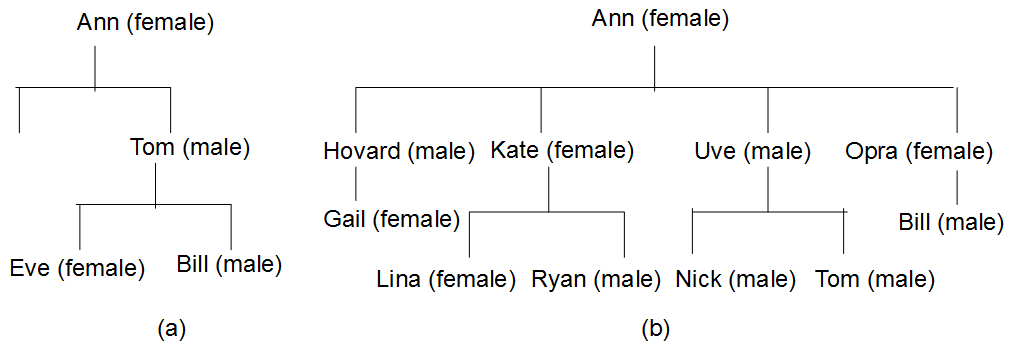
\includegraphics[bb =0 0 1055 346,scale =0.28]{tree_ds.png}
\caption{Two \emph{ancestor-descendant} trees.}
\end{figure}

In the second experiment to get the rule for the same target relation we used a more complex tree $ancestor-descendant$,  see Figure 2(b). The training data is following:
\begin{multline}\label{eq14}
\!\!\!\!\mathcal{B}=\! \{p(o, b), p(u, t), p(u, r), p(k, n), p(k, l), p(h, g), p(a, o), p(a, u), p(a, k), p(a, h),
f(a),\\
f(g), f(l), f(o), f(k)\}, \;
NegativeExamples=\!\! \{d(b, a), d(b, o), d(t, u), d(t, a), d(r, u), \\
d(n,k), d(n,a), d(r, a), d(l, a), d(g, a), d(u, a), d(h, a) \},\\
PositiveExamples= \{d(o, a), d(k, a), d(l, k), d(g, h) \},
\end{multline}
the person names also are denoted by initial letters and the same literal candidates are used.
The obtained rule is the same above. Indeed, Kate and Opra are Ann's daughters, Lina is Kate's daughter and Gail is Hovard's daughter; at the same time, for example, Tom is not a daughter of Kate or Ann,  Gail is not a daughter of Ann,  see Figure 2(b).

The goal of the third experiment was to build a rule for a target relation $son(X_1, X_2)$  based on training data shown at Figure 2(b) and we had to add a predicate $male(X)$ (denoted by letters $s$ and $m$). Here instead \eqref{eq13a} and \eqref{eq13b} we used
\begin{multline}\label{eq15}
\!\!\!\!\mathcal{B}=\! \{p(o, b), p(u, t), p(u, r), p(k, n), p(k, l), p(h, g), p(a, o), p(a, u), p(a, k), p(a, h),
m(b),\\m(u),m(t),m(r),m(n),m(h)\},\quad NegativeExamples= \{s(b, a), s(t, a), s(r, a), s(n, a),\\ s(l, a), s(g, a), s(o, a), s(k, a), s(l, k), s(g, h))\},\\
PositiveExamples= \{s(u, a), s(b, o), s(t, u), s(r, u), s(n, k), s(h, a)\},\\
candidates=\{
p(X_2, X_1), p(X_1, X_2), p(X_1, Y_1), p(Y_1, X_1), p(X_2, Y_1), p(Y_1, X_2),\\ p(X_1, X_1), p(X_2, X_2), m(X_1),m(X_2)\}.
\end{multline}
The obtained rule is the same above: $s(X_1, X_2)\leftarrow m(X_1)\; p(X_2, X_1)$. Indeed, Hovard and Uve are Ann's sons, Nick and Tom are Uve's sons,  Ryan is son of Kate and Bill is son of Opra. However, for example, Tom is not a son of Kate or Ann,  Ryan is not a son of Opra, Lina is not a son of Opra or Hovard,  see Figure 2(b).

\vspace{6pt}

\begin{tabular}{c}

\end{tabular}

Table 2. Efficiency indicators.

\begin{tabular}{|c|c|c|c|} %% viravnivanie: r po pravomu krau   c po centru
  \hline
  % after \\: \hline or \cline{col1-col2} \cline{col3-col4} ...
 No& Proportion of & Proportion of  & Running\\
Experiment &covered $\oplus (\%) $   examples&covered $\ominus$  examples (\%) &time (sec)\\
  \hline
1& 100 & 0 & 0.188 \\
    \hline
2& 100 & 0 & 0.207  \\
  \hline
3 & 100 & 0 & 0.200   \\
  \hline
 \end{tabular}

 \vspace{6pt}

All computations were performed on the computer with the following specifications:
Processor --- Intel(R) Core(TM) i5-7200; CPU 2.50GHz-2.70GHz;
Installed memory (RAM) = 8GB; System type --- 64-bit Operating System Windows 10 Home.

\section{Project timeline}

\emph{Author list:}

1. Georgiy Shurkhovetskyy --- Team leader; 2. Eskender Haziiev --- Team  member.


\vspace{3pt}

\begin{tabular}{|c|l|c|} %% viravnivanie: r po pravomu krau   c po centru
  \hline
Week & Planned work                     & Implementer \\
\hline
29.05.2017-11.06.2017 & Study of literature, writing project timeline    &  Team leader\\
& Study of literature, writing References &  Team member \\
\hline
11.06.2017-18.06.2017 & Building of algorithm structure & Team leader\\
& Progress presentation construction & Team member\\
\hline
19.06.2017-25.06.2017 & Building of data structure     &   Team leader\\
& Development of classes   & Team member \\
\hline
26.06.2017-02.07.2017 & Choice of effectiveness evaluation technique       &  Team leader\\
& Debugging the program   &   Team member \\
\hline
03.07.2017-09.07.2017 & Debugging the program     &   Team leader\\
&    & Team member\\
\hline
10.07.2017-16.07.2017 & Test 1 and evaluation of its results & Team leader   \\
& Test 2,3 and evaluation of its results & Team member  \\
\hline
17.07.2017-23.07.2017 & Writing 1,2,5 sections of the report  & Team leader \\
& Writing 3,4 sections of the report,  & Team member  \\
& Final presentation construction & Team member\\
\hline
\end{tabular}
\bibliographystyle{plainnat}
\bibliography{biblio}
\end{document}


